\section{Using BNNs Beyond Classification: Denoising binary Autoencoder}
Most of the works on BNN till date focus on classification tasks as a benchmark for evaluating the performance of BNNs. In this section we explore the usage of BNNs in  denoising auto encoder (AE), called Binary AE, referred as \textit{BAE}. The architecture we consider for this experiment is given in Table \ref{BAE}. Convolution represents 2D convolution layer for AE and quantized 2D convolution layer for BAE. Kernel size of convolution and deconvolution layers is $(3,3)$ and pool size of max pool layers is $(2,2)$ for both AE and BAE. In this AE architecture first three layers make up the encoder and last three the decoder part. At the first layer of the encoder and decoder, real valued inputs are used. STE-sign function is used as activation on current layer inputs for BAE except for the last layer. The last layer is a deconvolution layer with tanh activation. 
\begin{table}[ht]
  \caption{Architecture for Denoising Binary Auto Encoder}
  \label{BAE}
  \centering
  \begin{tabular}{lrcc}
    \hline
    Layer  &  No. of filters & Batch normalization & Activation on input\\
    \midrule
    Convolution + Maxpool &  $32$  & Yes & -  \\
    Convolution + Maxpool &  $16$  & Yes & STE-sign \\
    Convolution + Maxpool &  $8$  & Yes  & STE-sign \\
    Deconvolution + Upsampling2D &  $8$  & Yes  & - \\
    Deconvolution + Upsampling2D &  $16$  & Yes  & STE-sign \\
    Deconvolution + Upsampling2D &  $32$  & Yes  & STE-sign \\
    Deconvolution &  $3$  & Yes & tanh \\
    \bottomrule
  \end{tabular}
\end{table}
Mean square loss is minimized with BOP and a metric called peak signal to noise ratio (PSNR) is calculated to see the performance of the network during training and testing.
\begin{equation}
    PSNR = 10*\log_{10}\left(\frac{max^2}{mse}\right)
\end{equation}
where $max$ is the maximum possible pixel value of the image and $mse$ is the mean square error between original image and the image output from the network. For traditional AE, the architecture is exactly same except that each layer is trained on real weights with relu activation (instead of STE-sign in BAE) except for the last layer. As the architecture of AE is similar to binary AE except few changes, we do not repeat the architecture.
\begin{figure}[!ht]
    \centering
    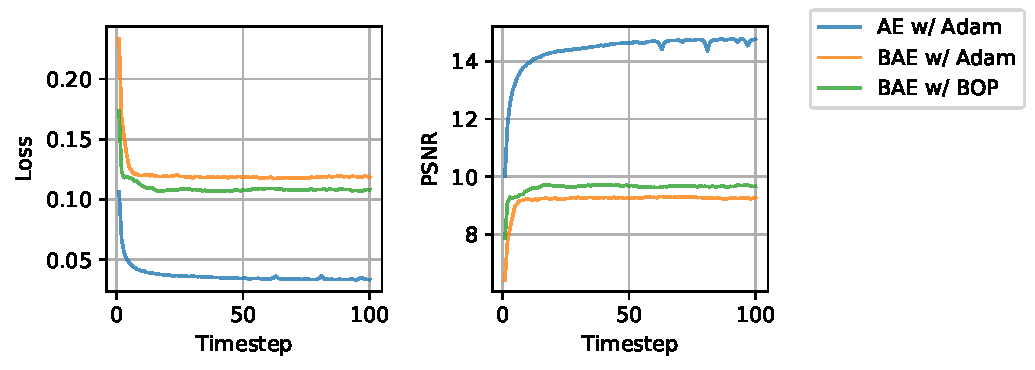
\includegraphics[scale=0.75]{fig/AEtradionalBNNBOP.pdf}
    \caption{Training PSNR (dB); At the end of training, PSNR for AE: $14.76$dB, BAE w/ Adam: $9.25$dB and BAE w/ BOP: $9.66$dB}
    \label{fig:AE}
\end{figure}


\begin{figure}[ht]
\centering
    \begin{subfigure}{0.98\textwidth}
        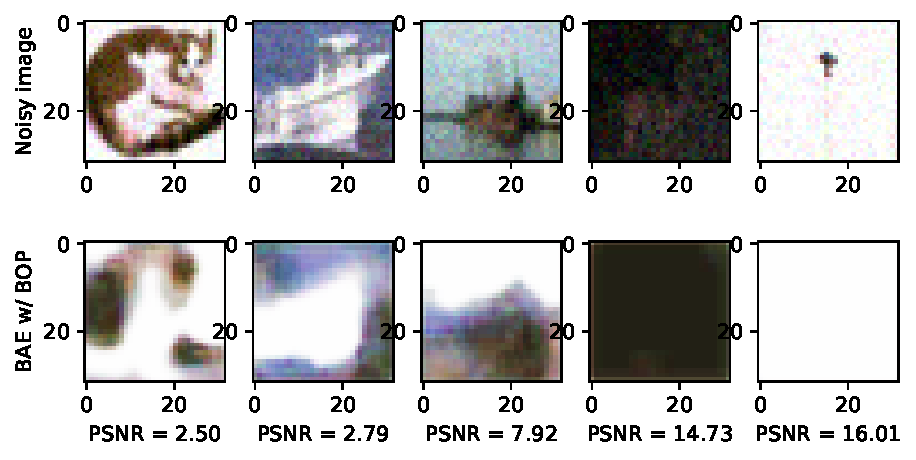
\includegraphics[width=1.\linewidth]{fig/BAEBOPfigsbestworst.pdf}
    \end{subfigure}
    \begin{subfigure}{0.98\textwidth}
        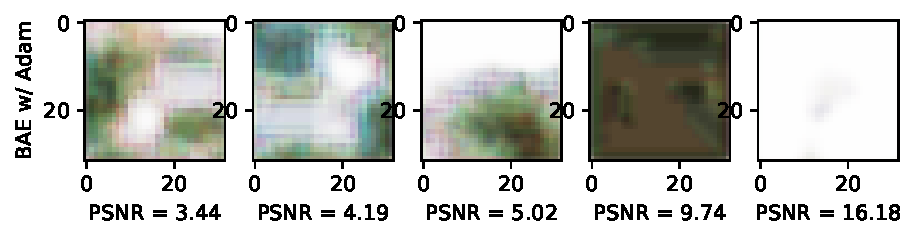
\includegraphics[width=1.\linewidth]{fig/BAEAdamfigsbestworst.pdf}
    \end{subfigure}
    \begin{subfigure}{0.98\textwidth}
        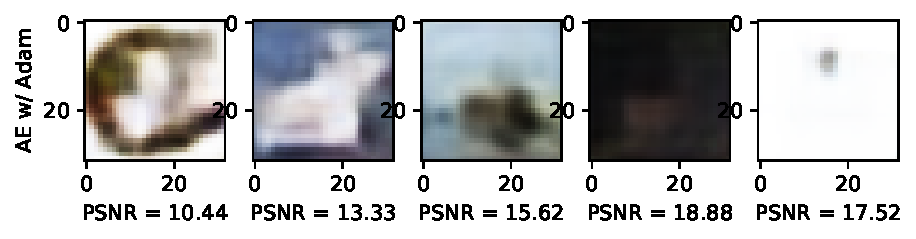
\includegraphics[width=1.\linewidth]{fig/AEAdamfigsbestworst.pdf}
    \end{subfigure}
    \caption{Comparison of recovered images by AE with Adam, BAE with Adam and BAE with BOP}
    \label{fig:AEfig}
\end{figure}

In order to use CIFAR10 dataset for training, we scale the $(32,32)$ images to $(-1,+1)$ say $im_{org}$. The shape of the images are referred as $im_{shape}$. Then a random normal $\mathcal{N}(0,1)$ noise is added with a noise factor $f = 0.1$ and the results are clipped between $(-1,+1)$ again resulting in a noisy image referred as $im_{noi}$.
\begin{equation}
    im_{noi} = \text{clip}\left((im_{org}+f* W), 0, 1\right) \qquad \text{ where } W \sim \mathcal{N}(0,1, im_{shape})
\end{equation}
We perform three sets of experiments, all using batch normalization to stabilize the training with a minibatch size of $64$. The sets are as follows:
\begin{enumerate}
    \item Traditional AE with Adam optimizer (with learning rate $lr = 10^{-3}$, $\beta_1 = 0.99$, $\beta_2 = 0.999$)
    \item BAE with Adam optimizer with same hyper parameters
    \item BAE with BOP optimizer ($\tau=10^{-8}, \gamma=10^{-5}$)
\end{enumerate}
In Fig \ref{fig:AE} the training loss and training PSNR is shown for all three cases. From the graphs we see that, BAE with BOP seems to be better than BAE with Adam for this task and the training converges faster. The test PSNRs of all three cases are as follows:
\begin{enumerate}
    \item AE with Adam: $14.87$ dB
    \item Binary AE with Adam: $9.10$ dB
    \item Binary AE with BOP: $9.30$ dB
\end{enumerate}
However, the results are not impressive for both of the BAE cases. We plot $5$ noisy samples of the CIFAR10 test dataset and the recovered images from the above three cases in Fig. \ref{fig:AEfig}. The reason behind degraded reconstructions for both of the BAE cases are: binary activations cannot pass enough information between the layers to develop a faithful reconstruction. Hence only a reduced finite set of information can be passed between intermediate layers of encoder and decoder. This could be the reason for not so good performance of BAE. We see a huge scope of improvement for BNN in case of BAE as well as other use cases.
